\documentclass{article}

\usepackage{graphicx}
\usepackage{tikz}
\usepackage{tikzsymbols}
\usetikzlibrary{calc,patterns,shapes.geometric}
\pagestyle{empty}
\usepackage[margin=0pt]{geometry}
\geometry{papersize={14in,12in}}

\def\centerarc[#1](#2)(#3:#4:#5){\draw[#1] ($(#2)+({#5*cos(#3)},{#5*sin(#3)})$) arc (#3:#4:#5);}

\begin{document}
	\begin{figure}
		\centering
		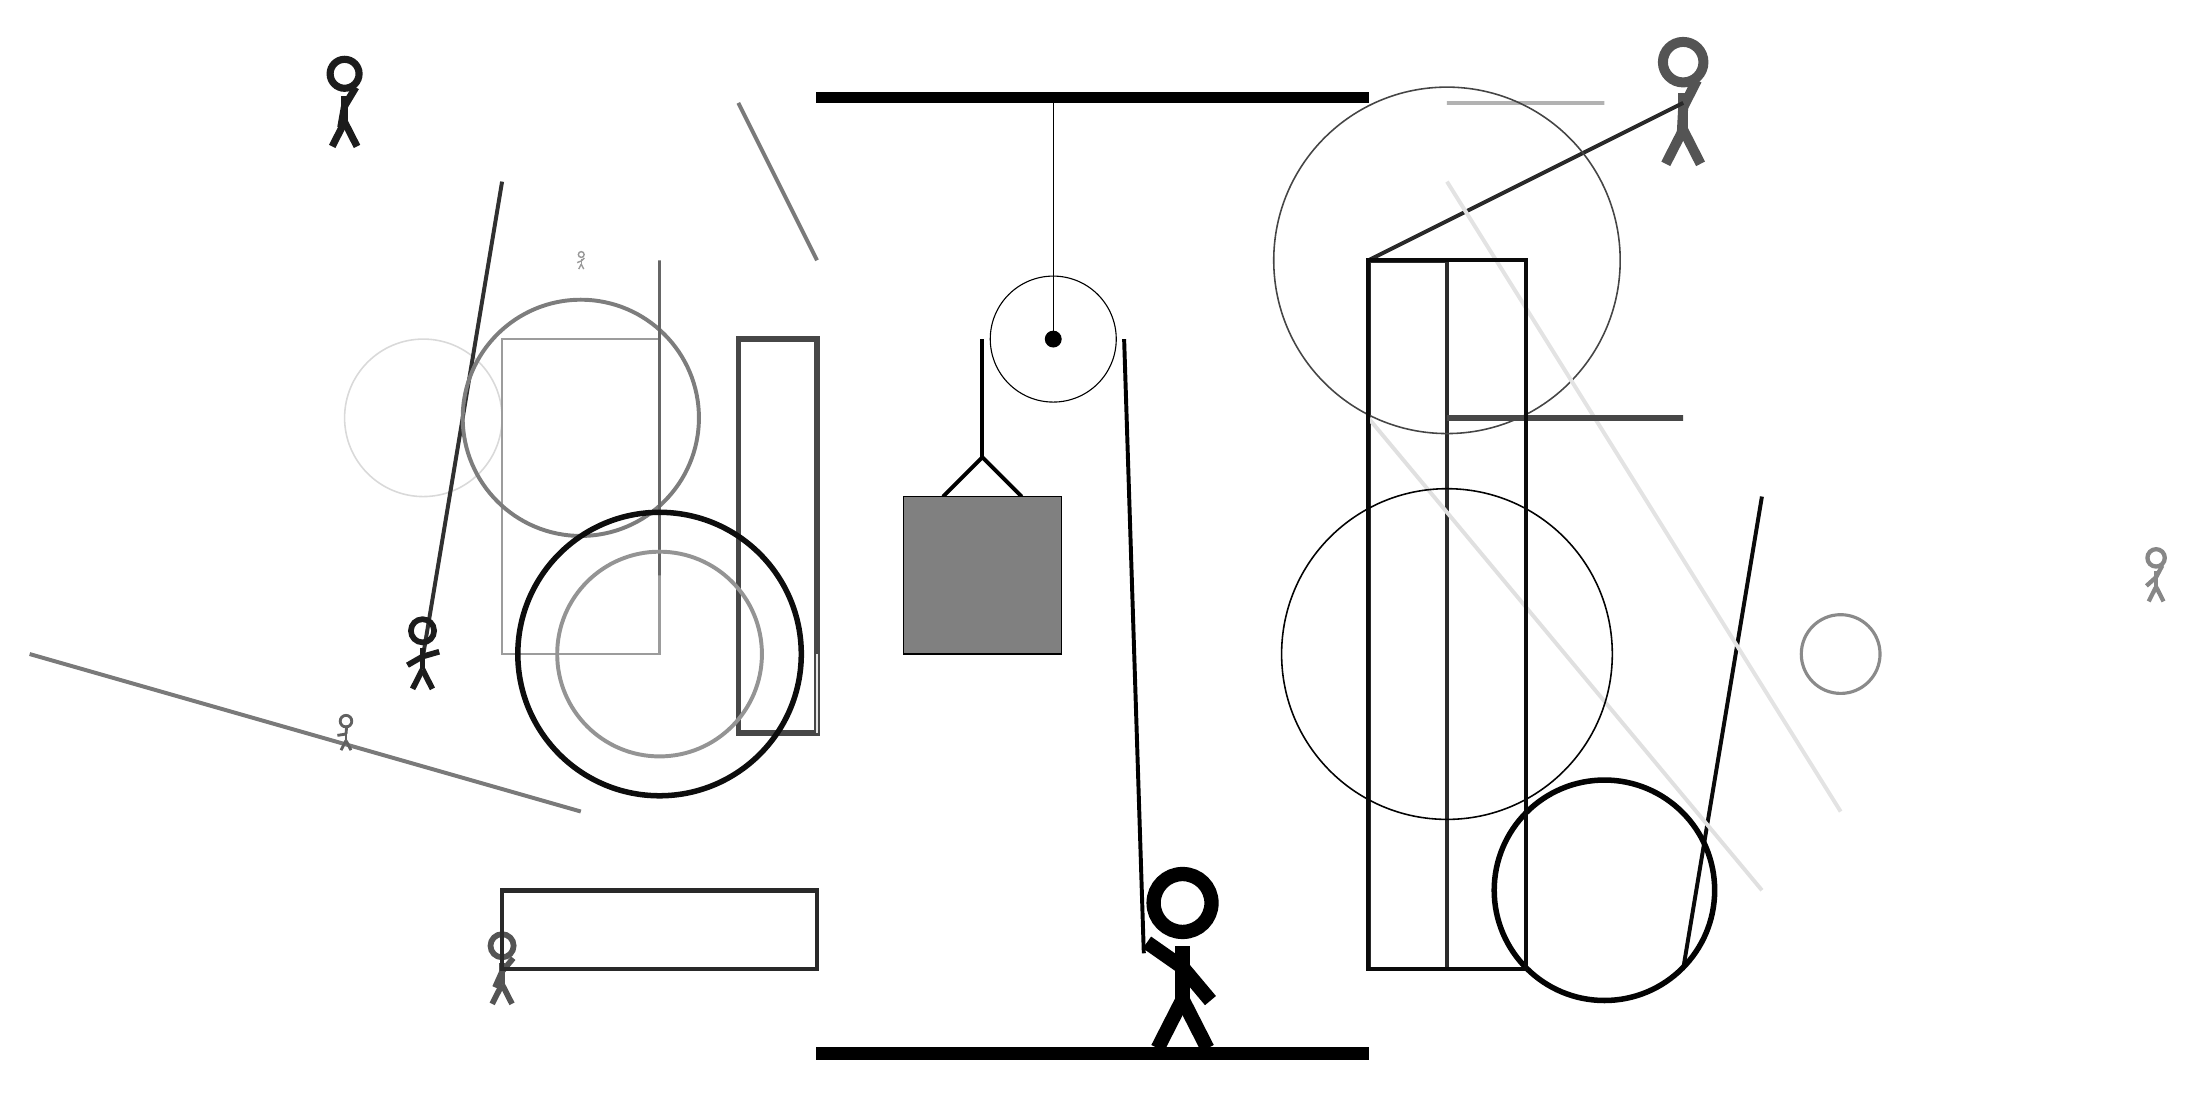
\begin{tikzpicture}
			%%%%% START %%%%%
			
			\draw[fill=black] (-2, 9) rectangle (5, 9.125);
			
			\draw (1, 6) circle (0.8);
			\draw[fill=black] (1, 6) circle (0.1);
			\draw (1, 9) -- (1, 6);
			
			\draw [line width=0.2mm, color=black!15](-7, 5) circle (1.0);
			
			\node[line width=0.2mm, color=black!67] at (9, 9) {\Strichmaxerl[7][87][63]};
			\draw[line width=0.5mm, color=black!81](-7, 2) -- (-6, 8);
			\draw [line width=0.6mm, color=black!14](9, 7) circle (0.0);
			
			\node[line width=0.5mm, color=black!89] at (-7, 2) {\Strichmaxerl[4][30][16]};
			\draw[line width=0.6mm, color=black!83] (5, 7) rectangle (6, -2);
			\draw[line width=0.5mm, color=black!30] (6, 9) rectangle (8, 9);
			\draw[line width=0.3mm, color=black!39] (-4, 2) rectangle (-6, 6);
			\draw[line width=0.5mm, color=black!96](9, -2) -- (10, 4);
			
			\draw[line width=0.5mm, color=black!52](-5, 0) -- (-12, 2);
			\draw [line width=0.5mm, color=black!51](-5, 5) circle (1.5);
			\draw[line width=0.5mm, color=black!84](9, 9) -- (5, 7);
			\node[line width=0.6mm, color=black!67] at (-6, -2) {\Strichmaxerl[4][66][50]};
			
			\node[line width=0.5mm, color=black!89] at (-8, 9) {\Strichmaxerl[5][80][59]};
			\draw [line width=0.4mm, color=black!46](11, 2) circle (0.5);
			\draw[line width=0.7mm, color=black!72] (-3, 1) rectangle (-2, 6);
			\draw[line width=0.3mm, color=black!60] (-4, 3) rectangle (-4, 7);
			\draw [line width=0.7mm, color=black!99](8, -1) circle (1.4);
			\draw[line width=0.5mm, color=black!52](-3, 9) -- (-2, 7);
			
			\draw [line width=0.5mm, color=black!42](-4, 2) circle (1.3);
			\draw[line width=0.6mm, color=black!84] (-2, -2) rectangle (-6, -1);
			
			\draw[line width=0.2mm, color=black!10] (-2, 1) rectangle (-2, 2);
			
			\draw [line width=0.2mm, color=black!73](6, 7) circle (2.2);
			\draw[line width=0.5mm, color=black!12](5, 5) -- (10, -1);
			\draw[line width=0.5mm, color=black!11](6, 8) -- (11, 0);
			
			\draw[line width=0.4mm, color=black!13] (7, 2) rectangle (7, 5);
			
			\draw[line width=0.7mm, color=black!72] (6, 5) rectangle (9, 5);
			\draw [line width=0.2mm, color=black!99](6, 2) circle (2.1);
			\node[line width=0.6mm, color=black!40] at (-5, 7) {\Strichmaxerl[1][22][43]};
			
			\node[line width=0.5mm, color=black!47] at (15, 3) {\Strichmaxerl[3][42][62]};
			\draw [line width=0.7mm, color=black!95](-4, 2) circle (1.8);
			
			\node[line width=0.2mm, color=black!62] at (-8, 1) {\Strichmaxerl[2][9][85]};
			\draw[line width=0.5mm, color=black!96] (7, -2) rectangle (5, 7);
			
			\draw[line width=0.5mm] (-0.4, 4.0) -- (0.1, 4.5) -- (0.6, 4.0);
			\draw[fill=black!50] (-0.9, 4.0) rectangle (1.1, 2.0);
			
			\draw[line width=0.5mm] (0.1, 6) -- (0.1, 4.5);
			\centerarc[line width=0.5mm](1, 6)(0:180:0.9);
			\draw[line width=0.5mm](1.9, 6) -- (2.15, -1.8);
			
			\node at (2.6, -1.9) {\Strichmaxerl[10][-35][-50]};
			
			\draw[fill=black] (-2, -3) rectangle (5, -3.15);
			
			%%%%% END %%%%%
		\end{tikzpicture}
	\end{figure}	
\end{document}